\chapter{Opis bazy mobilnej}

\section{Efektory}

\subsection{Dookólna baza jezdna}

Bazą sprzętową na której opiera się niniejsza praca jest dookólna baza mobilna. Jest to baza holonomiczna, która może poruszać się w dowolnym kierunku oraz zmienić swoją orientację w miejscu. Możliwe jest to dzięki zastosowaniu kół szwedzkich. Koła te umieszczone są w narożnikach prostokątnej platformy i napędzane są niezależnie przez serwomotory. Dzięki zamontowanym enkoderom możliwy jest odczyt odometrii robota. Opisywaną platformę przedstawia rysunek \ref{fig:omnivelma}.

\begin{figure}[H]
	\centering
	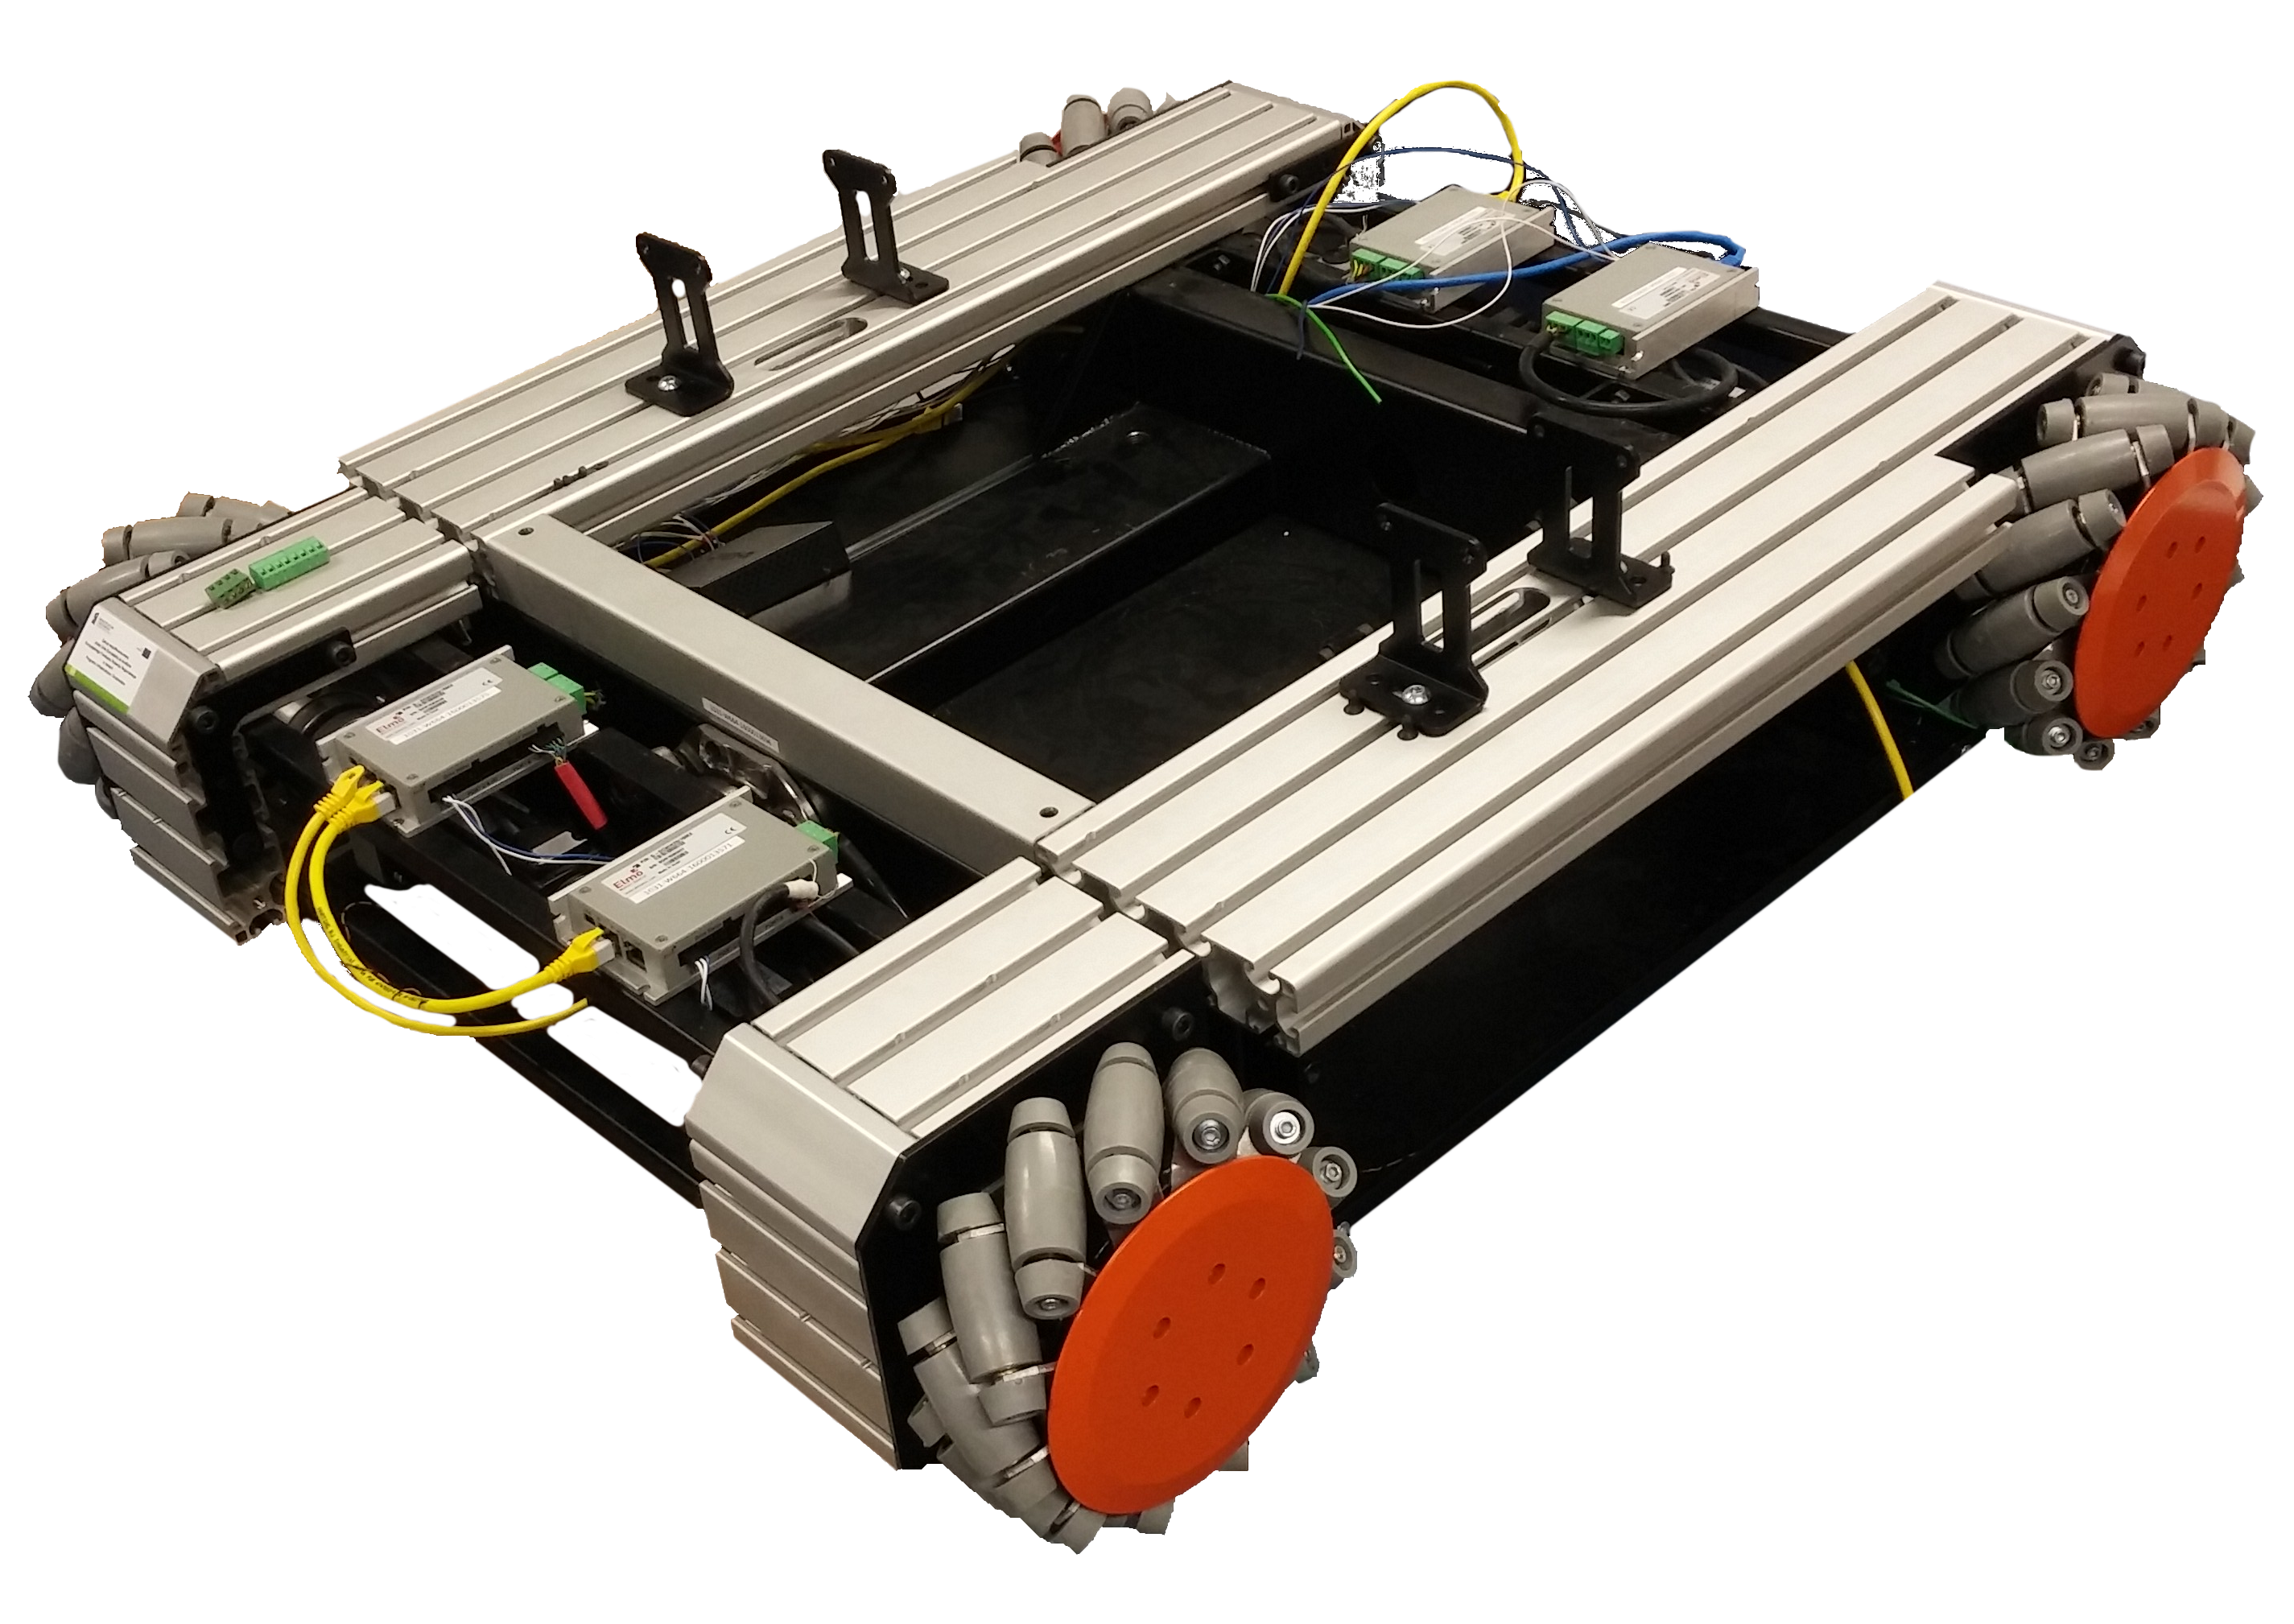
\includegraphics[width=0.6\textwidth]{gfx/omnivelma.png}
	\caption{Dookólna baza mobilna \cite{omnivelma}}
	\label{fig:omnivelma}
\end{figure}

Koła szwedzkie posiadają specjalne rolki ustawione pod kątem $45^{\circ}$ w stosunku do osi obrotu koła. Rolki te nie posiadają zdolności aktywnego ruchu, podążają jedynie za ruchem koła macierzystego. Ustawienie globalne kół, w znaczeniu skierowania rolek, na platformie odpowiada literze $X$, patrząc na platformę z góry \ref{fig:omnivelma}. Szkic kół szwedzkich można znaleźć na rysunku \ref{fig:wheels}.

\begin{figure}[H]
	\centering
	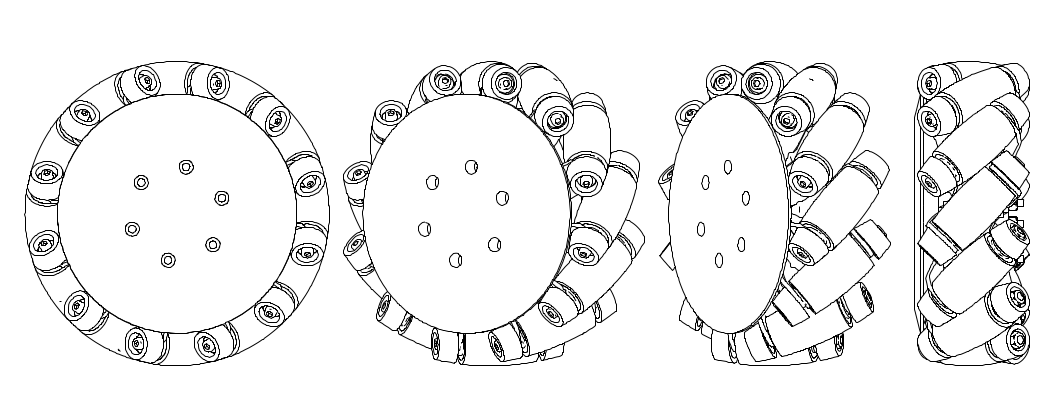
\includegraphics[width=0.5\textwidth]{gfx/wheels.png}
	\caption{Koła szwedzkie \cite{omnivelma}}
	\label{fig:wheels}
\end{figure}

Ruch platformy odbywa się poprzez odpowiednie zadawawanie prędkości każdemu z kół. Konstrukcja koła szwedzkiego powoduję, że koło to nie posiada tarcia w kierunku $45^{\circ}$ do osi obrotu macierzystego koła. Ma to istotne, gdyż siła jaka działa na koło jest prostopadła do tego kierunku (moment siły jest równoległy do osi koła). Konstrukcyjnie więc ustawiając koła w literę $X$ i odpowiednio manipulując wartościami prędkości dla każdego z kół, otrzymujemy możliwość ruchu w dowolnym kierunku \ref{fig:omnivelma}.

\begin{figure}[H]
	\centering
	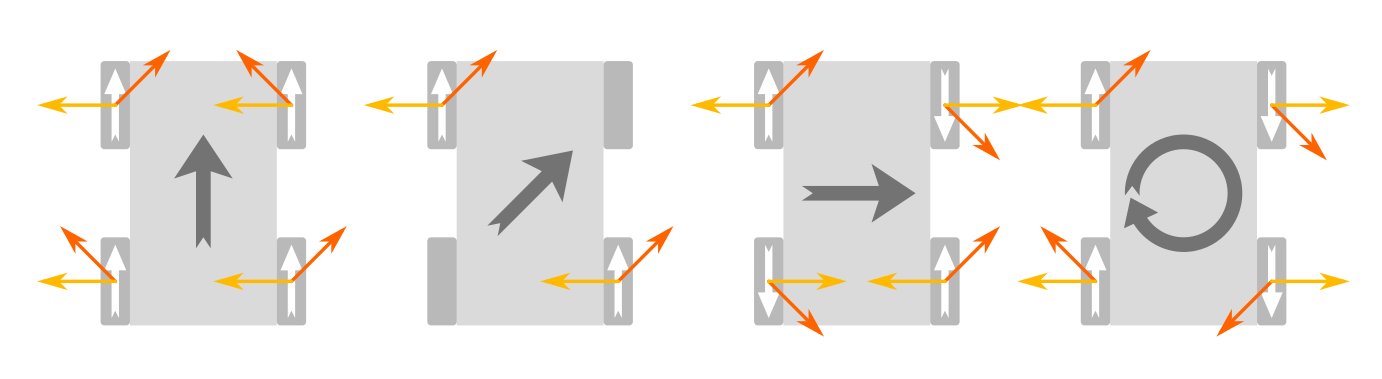
\includegraphics[width=0.8\textwidth]{gfx/vectors.png}
	\caption{Ruch platformy mobilnej - platforma widziana jest od góry, ciemna strzałka symbolizuję kierunek ruchu platformy, biała ruch koła, strzałka żółta to moment siły działający na dane koło, a czerwono-pomarańczowa to kierunek siły działającej na to koło \cite{omnivelma}}
	\label{fig:vectors}
\end{figure}

Z matematycznego punktu widzenia ruch platformy można opisać następującą macierzą, reprezentującą model kinematyki robota \ref{eq:kinematic}:

\begin{figure}[H]
  	\centering 
  	\begin{subfigure}[b]{0.4\textwidth}
  	\begin{equation} \label{eq:kinematic}
	\begin{bmatrix}
	v_x \\
	v_y \\
	\omega_z \\
	\end{bmatrix}
	=
	\frac{r}{4}
	\begin{bmatrix}
	-1 & 1 & -1 & 1 \\
	1 & 1 & 1 & 1 \\
	\frac{2}{a+b} & \frac{-2}{a+b} & \frac{-2}{a+b} & \frac{2}{a+b} \\
	\end{bmatrix}
	\begin{bmatrix}
	\omega_1 \\
	\omega_2 \\
	\omega_3 \\
	\omega_4 \\
	\end{bmatrix}
  	\end{equation}  
  	\caption{Równania kinematyki}
    \label{fig:kinematic_matrix} 
   	\end{subfigure}
  	\begin{subfigure}[b]{0.4\textwidth}
  		\centering
  		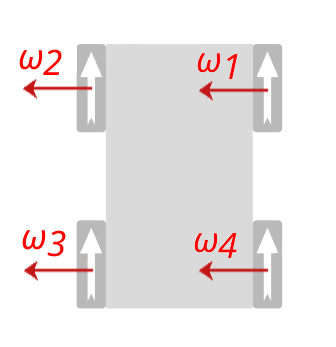
\includegraphics[height=3.5cm]{gfx/vectors2.png}
        \caption{Numeracja kół}
        \label{fig:n}
  	\end{subfigure}
  	\caption{Równania kinematyki robota oraz rysunek przedstawiający numeracje kół \cite{omnivelma}}
  	\label{fig:kinematic_main}
\end{figure}

Użycie platformy dookólnej w przedstawionej pracy ma głębokie uzasadnienie. Holonimiczność robota pozwala na elastyczne tworzenie trajektorii, bez narzutu ograniczeń ruchu bazy nieholonicznej. Przy bardzo bliskiej detekcji człowieka, bądź jego względnie dużej prędkości, system nie byłby w stanie stworzyć odpowiedniej trajektorii dla robota, co mogłoby powodać zatrzymanie ruchu do czasu oddalenie się osoby. Dodatkowo platforma dookólna ma ułatwione zadanie poruszania się w ciasnych przejściach, potrafi również obrócić się w miejscu. \\

Więcej na temat samej platformy przeczytać można w dedykowanej jej pracy \cite{omnivelma}.


\section{Receptory}

\subsection{Kinect}

Kinect jest sensorem wyprodukowanym przez Microsoft na potrzeby konsoli Xbox 360. Pierwotnym zadaniem była obsługa konsoli za pomocą gestów i poleceń głosowych oraz wykorzystanie w grach wideo. Jest również często wykorzystywany w robotyce ze względu na spore możliwości i niską cenę. Urządzenie składa się z promiennika podczerwieni oraz dwóch kamer - kamery wizyjnej RGB oraz kamery zwracającej informację o głębokości obrazu. Emiter podczerwieni emituję wiązke promieni podczerwonych, a kamera podczerwieni bada odbicia promieni od obiektów. Im obiekt jest bliżej, tym mocniejsze pada na niego światło. W ten sposób otrzymuję się chmurę punktów i interpolowany obraz głębi \cite{kinect}.

\begin{figure}[H]
	\centering
	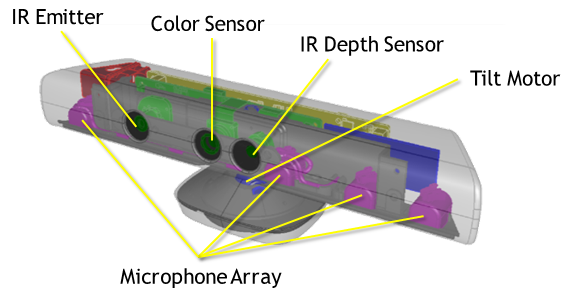
\includegraphics[width=0.8\textwidth]{gfx/kinect2.png}
	\caption{Budowa Kinecta - emiter podczerwieni, kamera RGB, sensor głębi, silnik i macierz mikrofonów \cite{kinect}}
	\label{fig:kinect}
\end{figure}

Kinect posiada również macierz mikrofonów, pozwalającą na realizację wykrywania komend użytkownika oraz silnik pozwalający na przechylanie Kinecta. Tabela przedstawia specyfikacje urządzenia.

\begin{table}[h]
\centering
{\renewcommand{\arraystretch}{1.5}
\begin{tabular}{ p{5cm} | p{7cm} }
 Rozdzielczość obrazu RGB & 640x480 \\
 \hline
 Rozdzielczość obrazu głębokości (interpolowana) & 300x200 (640x480) \\
 \hline
 Zakres pracy & 0.4m-6.5m \\
 \hline
 Pole widzenia & $43^{\circ}$ pionowo, $57^{\circ}$ poziomo \\
 \hline
 Klatki na sekunde (dla obu kamer) & 30 \\
 \hline
 Format audio & 16-kHz, 24-bit, modulacja PCM \\
 \hline
 Charakterystyka audio & Macierz czterech mikrofonów 24-bit, konwerter ADC, niwelacja echa i szumu
\end{tabular}}
\caption{Oficjalna specyfikacja Kinecta \cite{kinect}}
\label{tab:kinect_specification}
\end{table}

W procesie inżynierii wstecznej ustalono, że Kinect jest w stanie dostarczyć obraz RGB o rozdzielczości do 1280x1024, lecz przy zmniejszonej liczbie klatek na sekundę. Wysyła on także bezpośrednio (zanim zostanie skonwertowany na mapę błębokości) obraz z kamery IR w rozdzielczości 640x480, lub 1280x1024 przy zmniejszeniu liczby klatek na sekundę. Realny zakres pracy oceniono nna 1.2m-3.5m \cite{kinect_openkinect}. \\

Obraz RGB oraz dane o błębokości obrazu posłużą do wykrycia i ustalenia orientacji człowieka w przestrzeni. Baza mobilna sama w sobie nie posiada jednak zamontowanego Kinecta, co będzie poruszane w trakcie implementacji.\\

\subsection{LIDAR}

Zasada działania sensorów LIDAR opiera się na wysyłaniu wiązki laserowej i mierzenia czasu jej powrotu po odbiciu od przedmiotów. Na tej podstawie otrzymuję się informację o rozmieszczeniu przedmiotów w polu widzenia sensora. Wewnątrz sensora znajduje się ustawione pod kątem $45^{\circ}$ w stosunku do pionu lustro. Lustro zamontowane jest na silniku wraz z enkoderem. Urządzenie emituje wiązke laserową i na podstawie opóźnień w czasie powrotu wiązki do detektora oraz odometrii silnika (kąta jego obrotu) generuje się wyniki pomiarów \cite{lidar}. 


\begin{figure}[H]
	\centering
	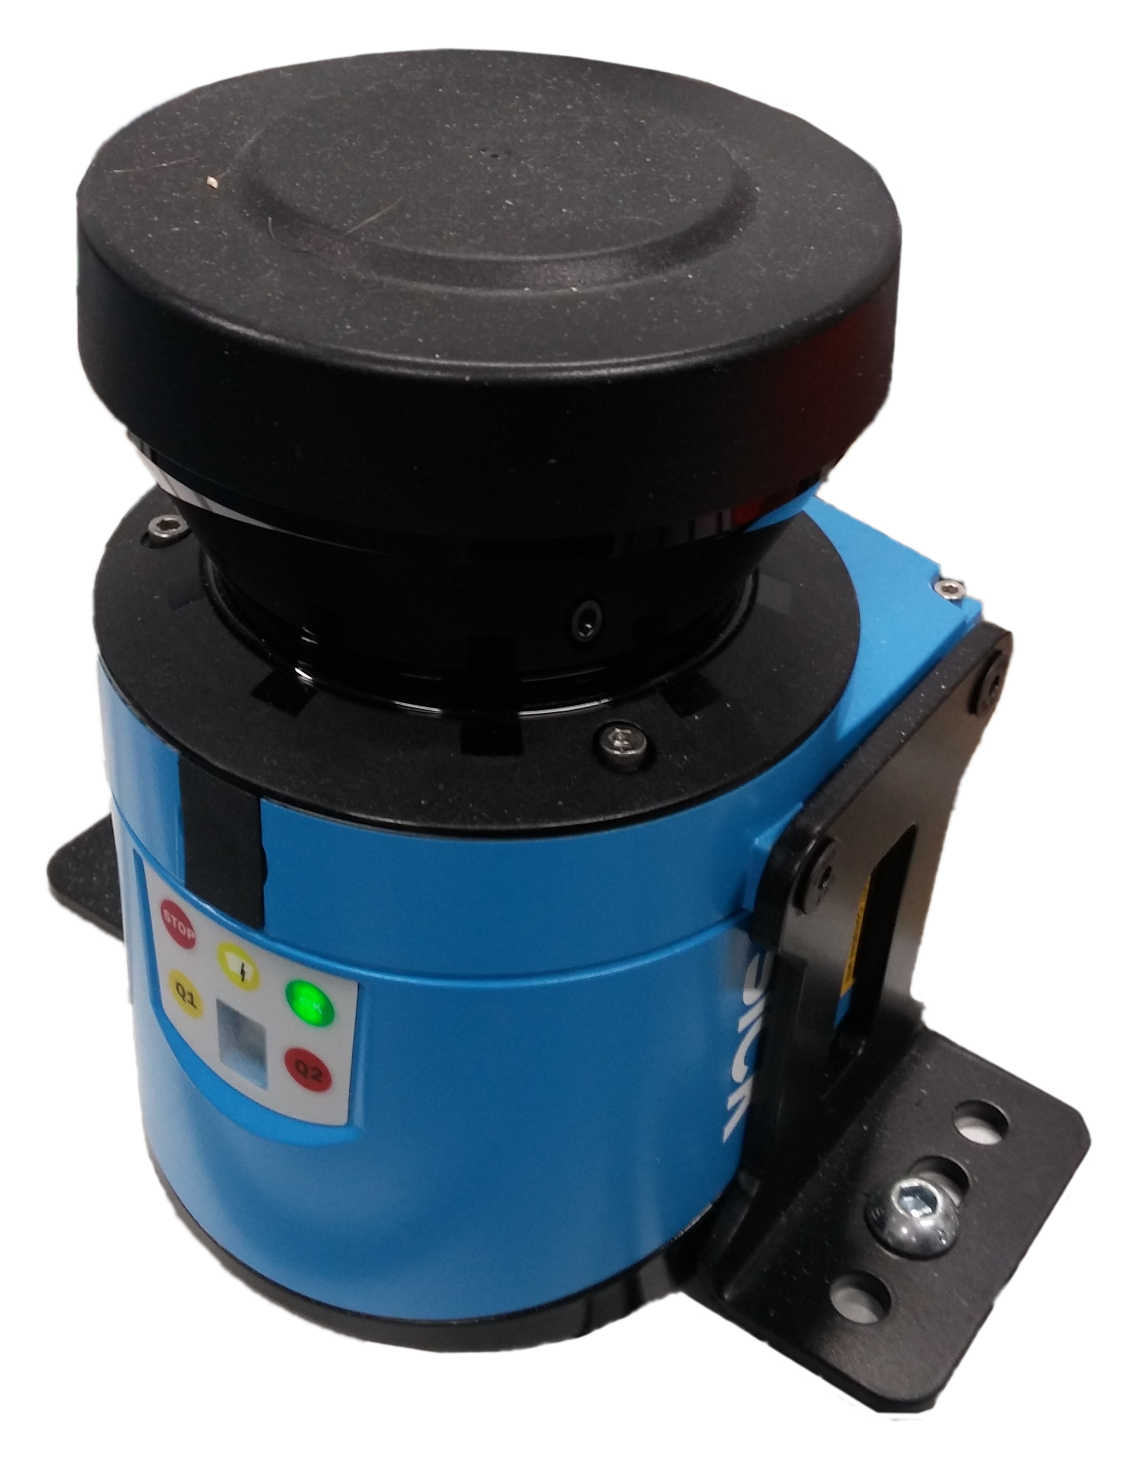
\includegraphics[width=0.4\textwidth]{gfx/lidar.png}
	\caption{LIDAR LMS100-1000 firmy SICK}
	\label{fig:sick}
\end{figure}


Platforma mobilna wyposażona jest w dwa sensory LIDAR LSM100-1000 firmy SICK \ref{fig:sick} \ref{tab:lidar_specification}, umiejscowione po jej przeciwnych stronach. Powodem zastosowania dwóch sensorów jest ograniczone pole widzenia jednego tylko sensora. Dwa sensory pozwalają na niemal dookólne mapowanie przestrzeni.

\begin{table}[h]
\centering
{\renewcommand{\arraystretch}{1.5}
\begin{tabular}{ p{8cm} | p{4cm} }
 Pole widzenia & $270^{\circ}$\\
 \hline
 Długość wykorzystanej fali lasera & 905nm (podczerwień) \\
 \hline
 Częstotliwość pracy & 50Hz \\
 \hline
 Maksymalna odległość pomiaru & 20m \\
 \hline
 Rozdzielczość pomiaru & $0.5^{\circ}$ \\
 \hline
 Systematyczny błąd pomiarowy & 0.03m \\
 \hline
 Przypadkowy błąd pomiaru odległości & 0.012m \\
\end{tabular}}
\caption{Specyfikacja sensora LIDAR LMS100-1000 firmy SICK \cite{omnivelma}}
\label{tab:lidar_specification}
\end{table}


Sensory LIDAR posłużą do tworzenia mapy środowiska, wykrywania przeszkód oraz detekcji człowieka.